\section{Validation of the Estimator and of the Intervals}
\label{sec:validation}
\emph{In short: pseudo-experiments generated from the fitted model show that the maximum-likelihood estimate of $A$ is unbiased and attains the minimum variance bound, that the Wilks interval has the nominal coverage, and that the test of $A=0$ has the expected size and a power that is known as a function of the injected asymmetry.}

The asymptotic properties of the maximum-likelihood estimator and of the profile-likelihood ratio were also verified on toy MC experiments generated from the fitted model of Sec.~\ref{sec:model} (Poisson yields, masses drawn from the model), as done for the Bayesian interval in Sec.~\ref{sec:bayes_toymc}: $1000$ experiments at the fitted value $A_{\mathrm{true}}=-0.0441$ and $300$ at each of $-0.1$, $-0.02$, $0$ and $+0.05$, each fitted with the nominal frequentist procedure ($1$--$3\%$ of the fits are not flagged valid by \texttt{MIGRAD} and are excluded).

\subsection{Bias, Efficiency and Coverage}
\label{sec:validation_estimator}
\emph{In short: no bias larger than $0.0008$, an estimator spread equal to the Hesse uncertainty within $6\%$, and coverage of $0.70\pm0.01$ and $0.95\pm0.01$ at the fitted value; the test of $A=0$ has size $0.051\pm0.013$ and power $0.68$ at $A=-0.02$.}
Table~\ref{tab:validation_toys} summarizes the estimator over the five injected values: the bias of $\hat A$ is at most $0.0008$ ($1.6$ standard errors), its spread equals the mean Hesse uncertainty within $6\%$ and the pulls have width $0.94$--$1.05$, so the estimator is unbiased and reaches the minimum variance bound. At the fitted value the coverage of $t(A_{\mathrm{true}})\leq1$ is $0.696\pm0.015$ ($68.3\%$ level) and $0.954\pm0.007$ ($95.4\%$ level); at $A_{\mathrm{true}}=+0.05$ the $68\%$ coverage is $0.614\pm0.028$, $2.5$ standard deviations low, not unexpected among five values.

\begin{table}[h]
\centering
\resizebox{\ifdim\width>\linewidth\linewidth\else\width\fi}{!}{\begin{tabular}{rrcccc}
\toprule
$A_{\mathrm{true}}$ & $n$ & bias & sd$(\hat A)/\langle\sigma_{\mathrm{Hesse}}\rangle$ & cov.\ $68\%$ & cov.\ $95\%$ \\
\midrule
$-0.1$ & $297$ & $-0.0005\pm0.0005$ & $0.94$ & $0.71$ & $0.96$ \\
$-0.0441$ & $985$ & $-0.0001\pm0.0003$ & $0.97$ & $0.70$ & $0.95$ \\
$-0.02$ & $290$ & $-0.0008\pm0.0005$ & $1.02$ & $0.69$ & $0.94$ \\
$0$ & $293$ & $+0.0002\pm0.0005$ & $1.01$ & $0.69$ & $0.95$ \\
$+0.05$ & $293$ & $-0.0004\pm0.0005$ & $1.05$ & $0.61$ & $0.96$ \\
\bottomrule
\end{tabular}}
\caption{Pseudo-experiments at five injected values of the asymmetry: number of valid fits, bias of $\hat A$ with its standard error, spread of the estimates relative to the mean Hesse uncertainty ($0.0085$), and coverage of the intervals $t(A_{\mathrm{true}})\leq1$ and $\leq3.84$.}
\label{tab:validation_toys}
\end{table}

\emph{Size and power.} Under $A_{\mathrm{true}}=0$ the test $q(0)>3.84$ rejects in $0.051\pm0.013$ of the toy experiments, the nominal size, and $q(0)$ is compatible with $\chi^2_1$ (Kolmogorov-Smirnov $p=0.79$). Figure~\ref{fig:validation_power} gives the power: $1.00$ at the fitted value and $0.68$ ($0.27$ at $3\sigma$) at $A_{\mathrm{true}}=-0.02$, so with $19{,}731$ candidates an asymmetry below $\sim0.02$ is not resolved. The $5.2\sigma$ of the data is an extrapolation of the $\chi^2_1$ tail, which the $293$ experiments check only down to the $3\sigma$ level (Sec.~\ref{sec:validation_power}).

\begin{figure}[t]
\centering
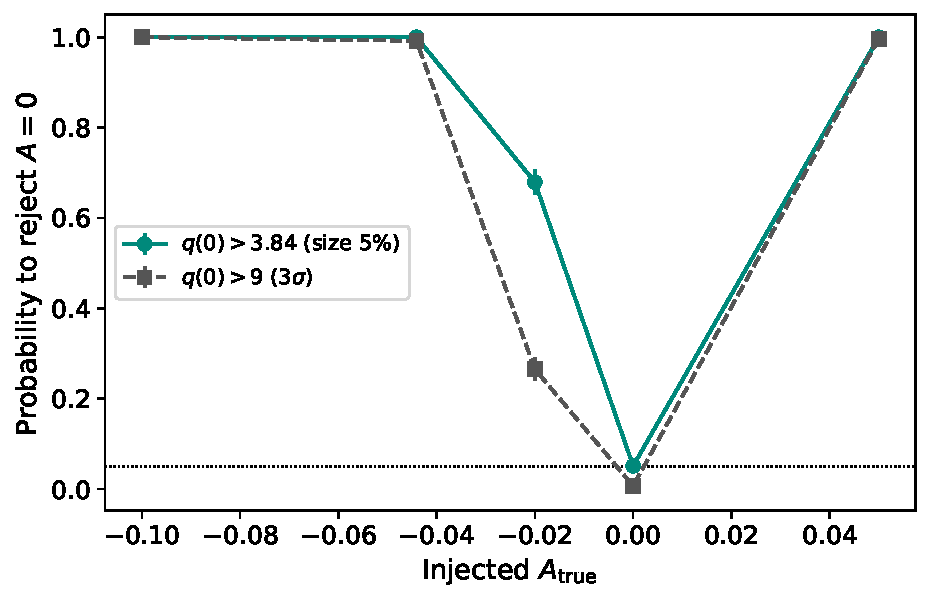
\includegraphics[width=\columnwidth]{figures/validation_power.pdf}
\caption{Probability to reject $A=0$ as a function of the injected asymmetry, with the test $q(0)>3.84$ (size $5\%$, dotted line) and $q(0)>9$ ($3\sigma$); $1000$ toy experiments at $-0.0441$, about $300$ at each other value.}
\label{fig:validation_power}
\end{figure}

\begin{figure*}[!t]
\centering
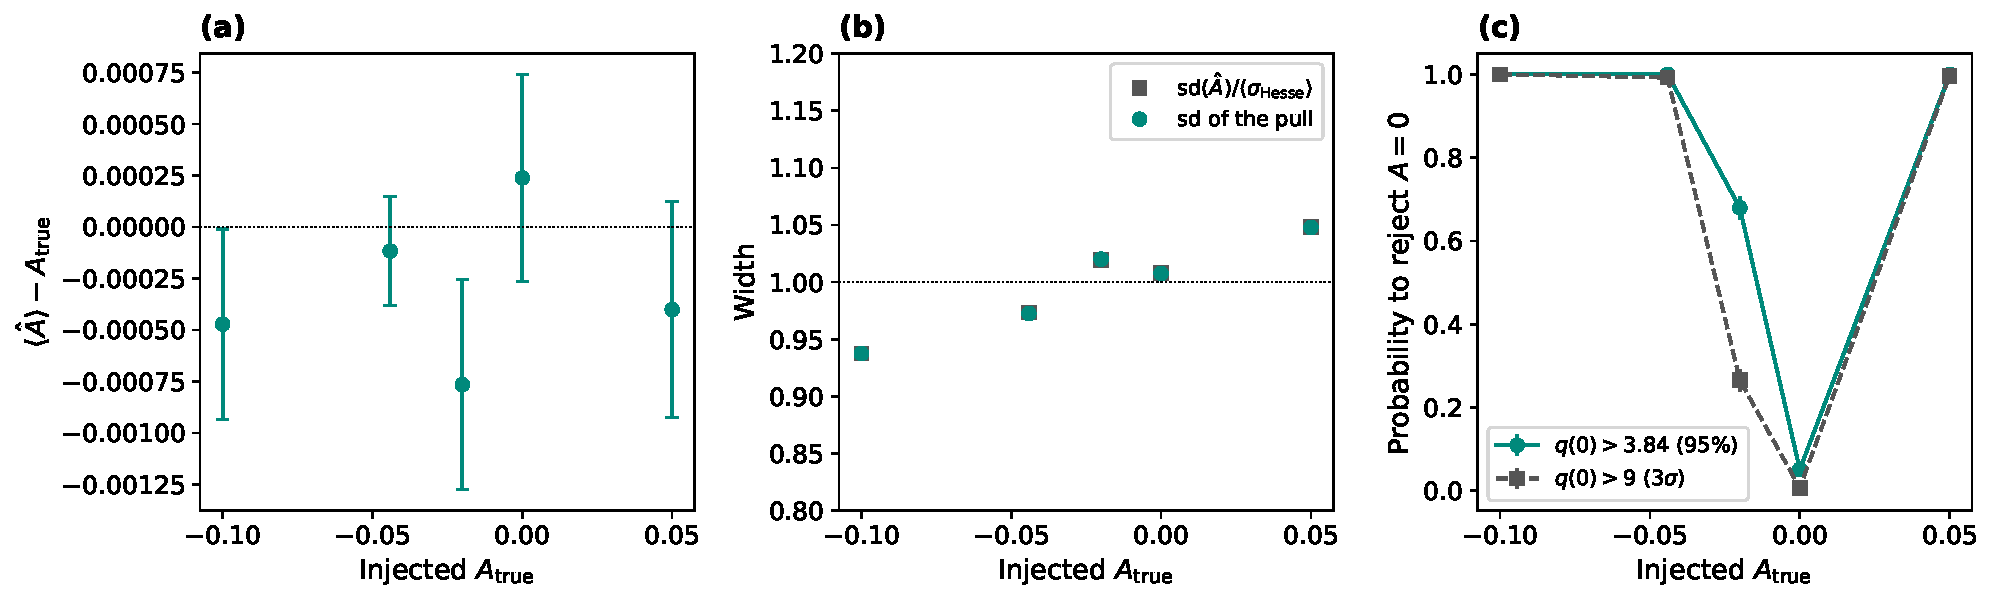
\includegraphics[width=0.95\textwidth]{figures/validation_injection_power.pdf}
\caption{Pseudo-experiments at five injected asymmetries. (a) Bias of $\hat A$, with its standard error. (b) Spread of the estimates divided by the mean Hesse uncertainty, and width of the pulls. (c) Probability to reject $A=0$ in the test with $q(0)>3.84$ (size $5\%$) and $q(0)>9$ ($3\sigma$), as a function of the injected value: size at $A_{\mathrm{true}}=0$, power elsewhere.}
\label{fig:validation_injection}
\end{figure*}

\begin{figure*}[!t]
\centering
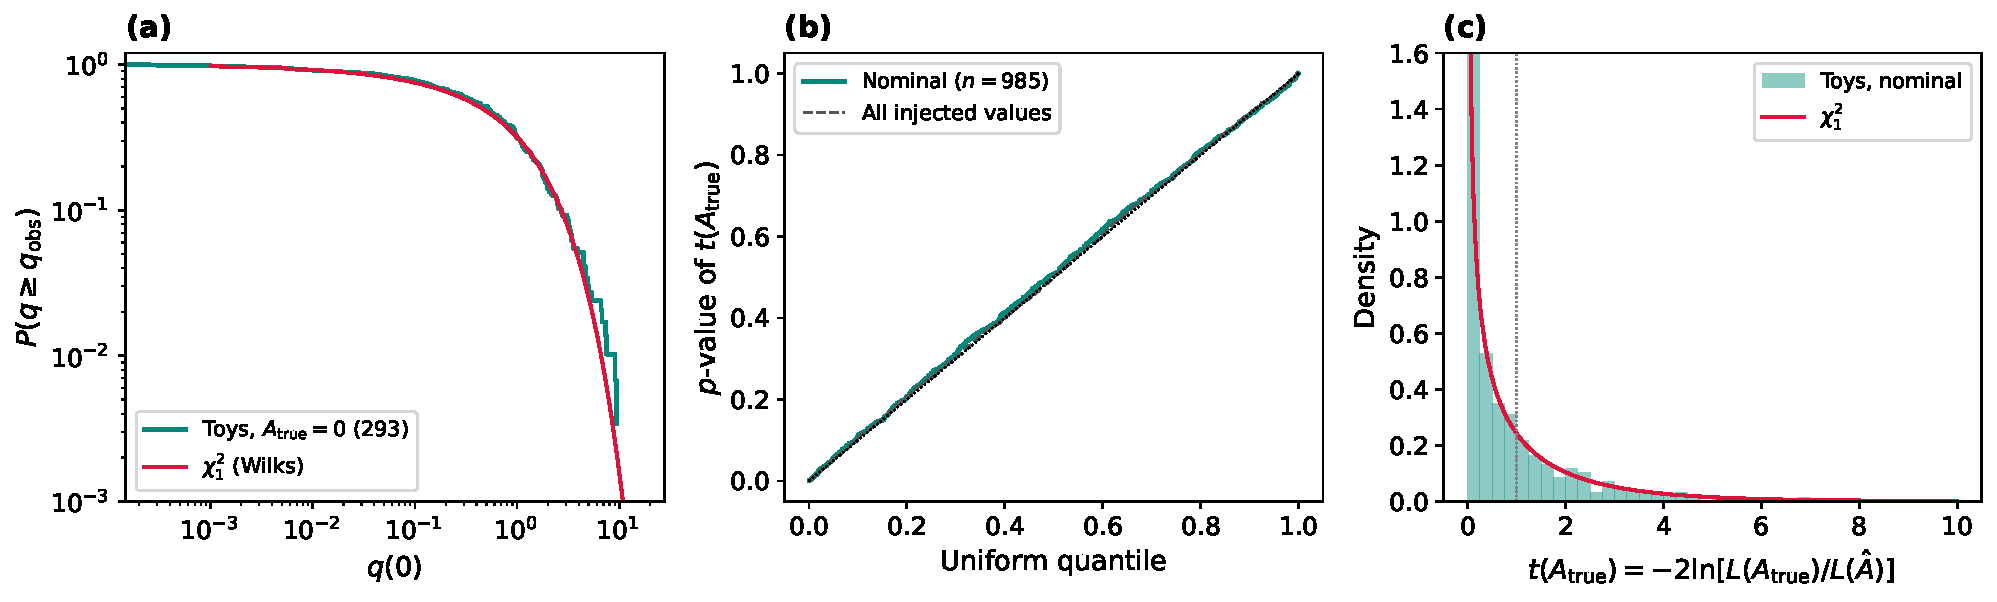
\includegraphics[width=0.95\textwidth]{figures/validation_null_wilks.pdf}
\caption{Pseudo-experiments, validity of Wilks' theorem. (a) Fraction of experiments with $q(0)$ above the observed value, for $A_{\mathrm{true}}=0$, compared with the $\chi^2_1$ distribution. (b) $p$-value of $t(A_{\mathrm{true}})$ against a uniform distribution, at the fitted value and pooled over the injected values. (c) Distribution of $t(A_{\mathrm{true}})$ at the fitted value and $\chi^2_1$.}
\label{fig:validation_null}
\end{figure*}

\subsection{Size and Power of the Test of $A=0$}
\label{sec:validation_power}
\emph{In short: the test has the nominal size, the statistic $q(0)$ follows a $\chi^2$ distribution with one degree of freedom, and an asymmetry of $-0.02$ would be rejected at $3\sigma$ in one pseudo-experiment out of four.}
Under $A_{\mathrm{true}}=0$ the fraction of pseudo-experiments with $q(0)>3.84$ is $0.051\pm0.013$, against the nominal size $\alpha=0.05$, and $2$ of $293$ exceed $q=9$ ($3\sigma$), against the $0.8$ expected; the distribution of $q(0)$ is compatible with $\chi^2_1$ (Kolmogorov-Smirnov $p=0.79$, Fig.~\ref{fig:validation_null}a), and the tail used for the significance ($q=27$) is an extrapolation of it. The power, the probability of rejecting $A=0$ when the asymmetry is $A_{\mathrm{true}}$ (Fig.~\ref{fig:validation_injection}c), is $1.00$ at the fitted value and at $\pm$ the larger injected values, and $0.68$ ($0.27$ at $3\sigma$) at $A_{\mathrm{true}}=-0.02$: with $19{,}731$ candidates an asymmetry of $0.02$ is detected in about two experiments out of three at the $5\%$ size, and an asymmetry below that is not resolved.


\subsection{Goodness of Fit and the Binning}
\label{sec:validation_gof}
\emph{In short: the binned $\chi^2$ of pseudo-experiments follows its asymptotic distribution, so its $p$-values are accurate; the misfit of the data is $5.4$ standard deviations at $10\,\MeV$ bins and $2.0$ at $2.5\,\MeV$, because it lives on the scale of the flanks of the peak.}
The $p$-values of the binned $\chi^2$ rely on the asymptotic distribution with $\mathrm{ndof}$ degrees of freedom, which can fail for bins with few entries. The $\chi^2$ of $1000$ pseudo-experiments from the fitted model has mean $87.6$ and standard deviation $13.3$ for $2\times50$ bins ($88$ degrees of freedom, expected $\sqrt{2\cdot88}=13.3$), and mean $387.6$, standard deviation $27.1$ for $2\times200$ bins ($388$ degrees of freedom): the asymptotic $\chi^2$ distribution describes the toys (Fig.~\ref{fig:validation_gof}). The data give $159.5$ for $2\times50$ bins of $10\,\MeV$, $5.4$ standard deviations above the toys (asymptotic $p=4.8\times10^{-6}$, fewer than $1/1000$ toys above), $253.1/188$ for $5\,\MeV$ bins ($p=1.1\times10^{-3}$) and $441.7/388$ for $2.5\,\MeV$ bins ($2.0$ standard deviations, $p=0.031$, in toys $0.032$). The same fit therefore has $p=0.03$ or $p=5\times10^{-6}$ depending on the binning: the discrepancy between model and data is a feature of $\sim10\,\MeV$ width, the flanks of the peak (Fig.~\ref{fig:bayes_fit}), diluted in narrower bins, and the binned $\chi^2$ is a test whose power depends on the binning, in the same way as the Bayes factor depends on the prior width.

\begin{figure*}[!t]
\centering
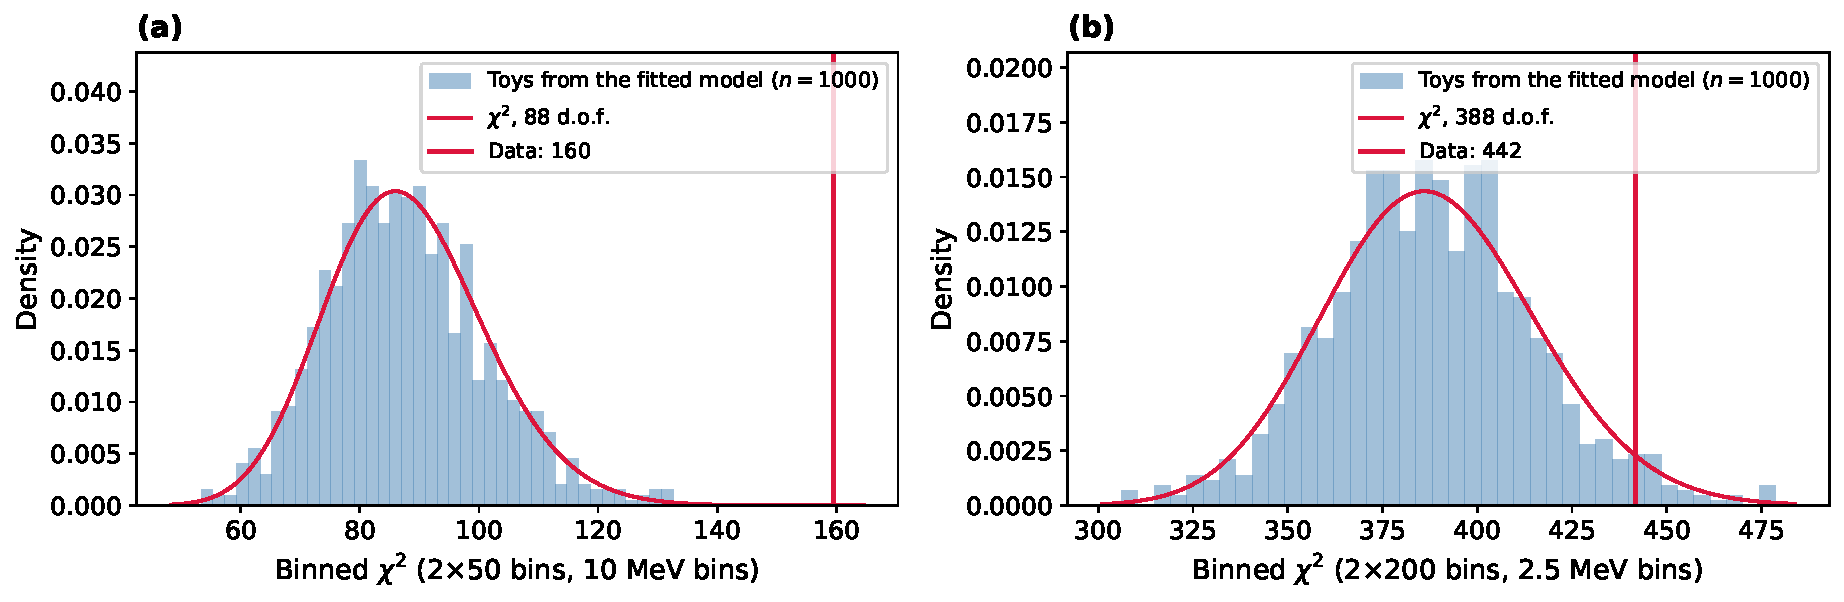
\includegraphics[width=0.95\textwidth]{figures/validation_gof_toys.pdf}
\caption{Binned $\chi^2$ of $1000$ pseudo-experiments from the fitted model, $\chi^2$ distribution with the corresponding degrees of freedom, and value of the data: (a) $2\times50$ bins of $10\,\MeV$, (b) $2\times200$ bins of $2.5\,\MeV$.}
\label{fig:validation_gof}
\end{figure*}
